\section{Backtracking} \label{sec:backtracking}

Backtracking é um tipo de algoritmo que representa um refinamento da busca por força bruta,
em que múltiplas soluções podem ser eliminadas sem serem explicitamente examinadas. O termo
foi cunhado pelo matemático estado-unidense D. H. Lehmer na década de 1950.

O procedimento é usado em linguagens de programação como Prolog. Uma busca inicial 
em um programa nessa linguagem segue o padrão busca em profundidade, ou seja, a árvore
é percorrida sistematicamente de cima para baixo e da esquerda para direita. Quando essa
pesquisa falha, ou é encontrado um nodo terminal da árvore, entra em funcionamento o
mecanismo de backtracking. Esse procedimento faz com que o sistema retorne pelo mesmo 
caminho percorrido com a finalidade de encontrar soluções alternativas. 

\subsection{Problema do labirinto}

\begin{figure}[ht]
  \centering
  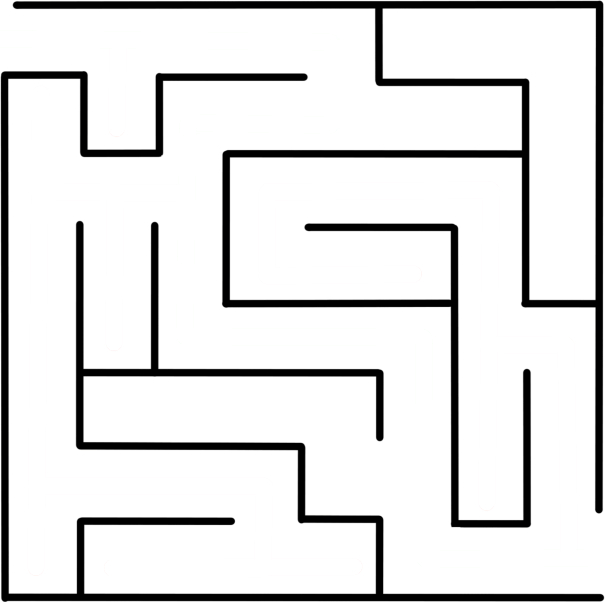
\includegraphics[width=.3\textwidth]{labirinto.jpg}
  \caption{Um exemplo de labirinto}
  \label{fig:labirinto}
\end{figure}

Problema do labirinto